\documentclass[utf8, a4paper, 11pt]{beamer}

\usepackage[english]{babel}
\usepackage[T1]{fontenc}

\usepackage{amsmath, amsfonts, wrapfig, graphicx}
\usepackage{bm}
\usepackage{mathtools}

\usepackage{beamerthemesplit}
\usetheme{CambridgeUS}

\setbeamertemplate{footline}
{\leavevmode%
  \hbox{%
  \begin{beamercolorbox}[wd=\paperwidth,ht=2.25ex,dp=1ex,right]{date in head/foot}%
    \usebeamerfont{date in head/foot}\insertshortdate{}\hspace*{2em}
    \insertframenumber{}-\inserttotalframenumber\hspace*{2ex} \end{beamercolorbox}}%
}

\setbeamertemplate{navigation symbols}{}  % Remove navigation bear

\newtheorem{innercustomgeneric}{\customgenericname}
\providecommand{\customgenericname}{}
\newcommand{\newcustomtheorem}[2]{%
  \newenvironment{#1}[1]
  {%
   \renewcommand\customgenericname{#2}%
   \renewcommand\theinnercustomgeneric{##1}%
   \innercustomgeneric}
  {\endinnercustomgeneric}
}

\newcustomtheorem{thm}{Theorem}
\newcustomtheorem{lem}{Lemma}
\newcustomtheorem{cor}{Corollary}
\newcustomtheorem{deftn}{Definition}
\newcustomtheorem{prop}{Proposition}
\DeclareMathOperator*{\argmin}{argmin}
\DeclareMathOperator*{\dist}{dist}
\DeclareMathOperator*{\argmax}{argmax}
\DeclareMathOperator*{\Tr}{Tr}

\title{On the representation of sphere-like surfaces with splines}
\institute[Uhlmann's lab]{\textbf {V. Uhlmann's lab}}
\author{Yoann Pradat}
\date{\today}
\titlegraphic{
\includegraphics[width=4cm]{EMBL_EBI-logo.png}}

\begin{document}


\frame{\titlepage}

\section[Outline]{}
\frame{\tableofcontents}

\section{Introduction}

\frame{\frametitle{Framework and motivation}
  Unkown function $g: \mathbb{R}^d \to \mathbb{R}^d, \mathbb{R}^{d+1}$ to be reconstructed from \textbf{finite} set of 
  values 
  
  \begin{enumerate}
    \item $g(\mathbf{t_1}), \ldots, g(\mathbf{t_n})$
    \item Possibly $\partial^{\bm{\alpha}} g(\mathbf{t_1}), \ldots, \partial^{\bm{\alpha}} g(\mathbf{t_n})$ with 
      $\bm{\alpha} \in \mathbb{N}^d$
  \end{enumerate}
  General model for the approximation $f$ to $g$ 
  \begin{equation}
    f(t) = \sum_{k} c_k^T \Phi(t-t_k) 
  \end{equation}
}

\frame{\frametitle{Example applications}
  \begin{footnotesize}
  1D $g:\mathbb{R} \to \mathbb{R}$. Known values $g(0), \ldots, g(9)$.  \\ 
  2D $r=g:\mathbb{R} \to \mathbb{R}^2$.  Known values $r(0), \ldots, r(3)$, $\partial^{1} r(0), \ldots, \partial^{1} 
  r(3)$ \\
  3D $\sigma=g:\mathbb{R}^2 \to \mathbb{R}^3$. Known values $\sigma(k,l), \partial^{1,0} \sigma(k,l), \partial^{0,1} 
  \sigma(k,l), \partial^{1,1} \sigma(k,l)$.

  \end{footnotesize}
   
  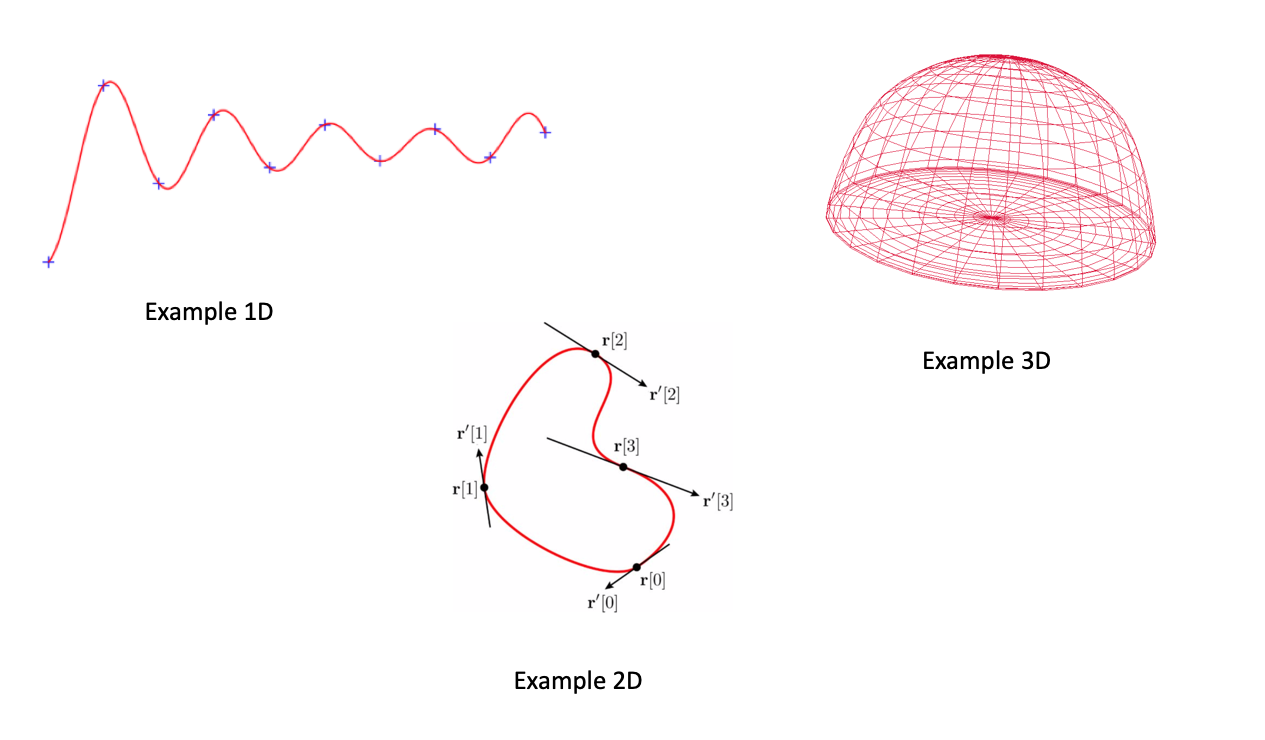
\includegraphics[width=0.9\linewidth]{examples.png}
}

\section{I/ Introduction to interpolation}
\subsection{I/1 Polynomial interpolation}
\frame{\frametitle{Lagrange polynomials}
  Denote $\Pi_{<k}$ set of polynomials of order $k$ (vector space). \\
  \underline{Obj}: reconstruct $g:\mathbb{R} \to \mathbb{R}$ from $g(t_1), \ldots, g(t_n)$.  \begin{thm}{1}
    Given $n$ sites (not necessarily distinct), there exists a unique $f$ in $\Pi_{<n}$ that agrees with $g$ at 
    ${(t_i)}_1^n$.
  \end{thm}
  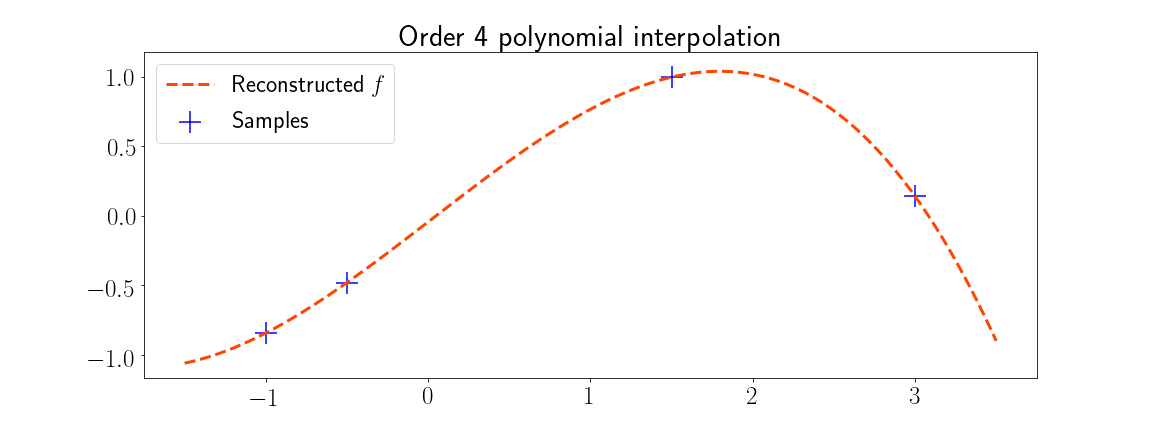
\includegraphics[width=0.9\linewidth]{lagrange_1.png}
}

\frame{\frametitle{Simply choose $n$ big enough?}
  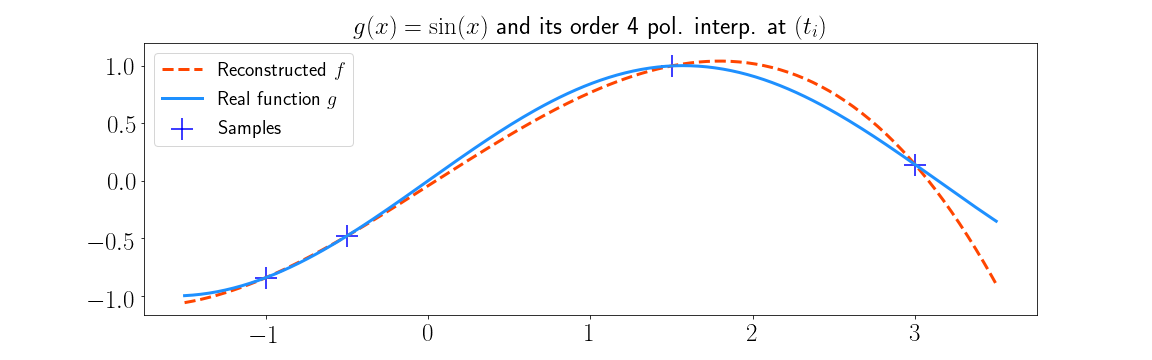
\includegraphics[width=0.9\linewidth]{lagrange_2.png}\vfill
  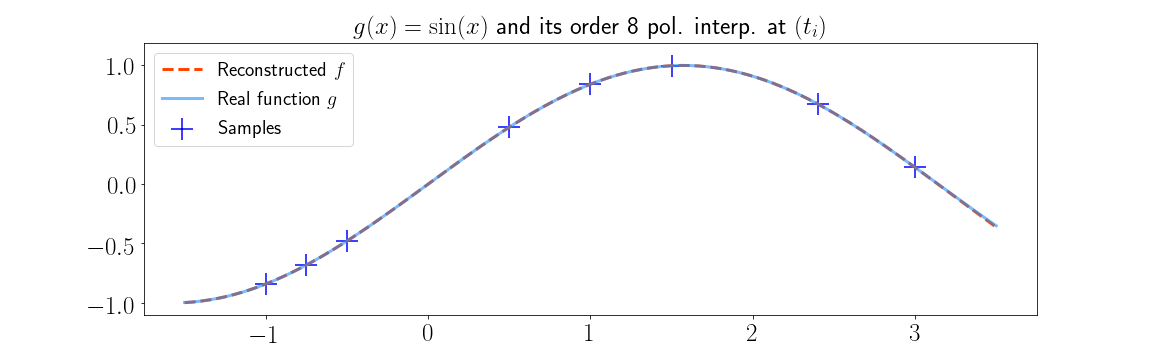
\includegraphics[width=0.9\linewidth]{lagrange_3.png}

  Take sufficiently many points and all is well?
}

\frame{\frametitle{Runge example}
  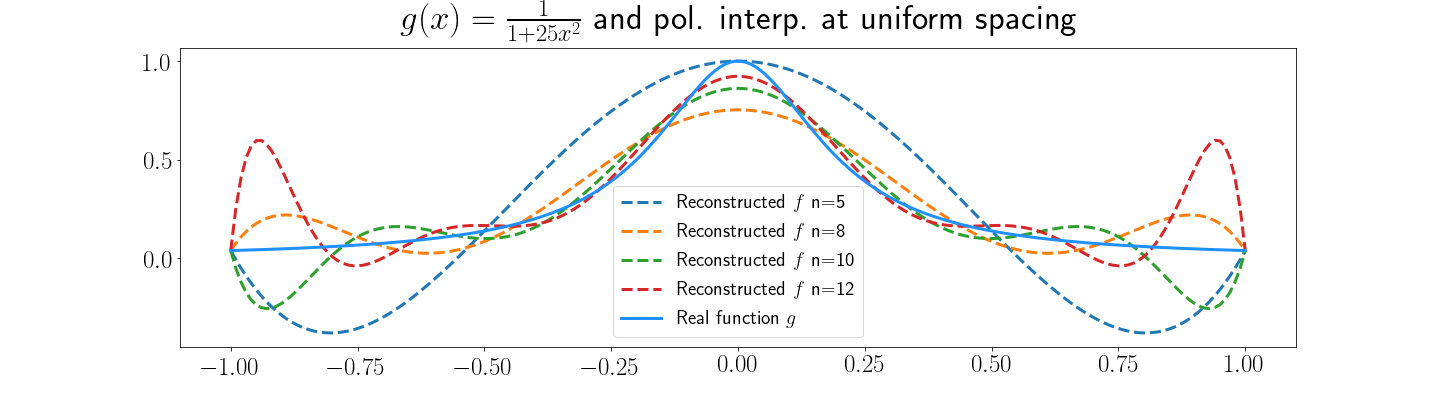
\includegraphics[width=\linewidth]{runge_1.png}
  \begin{footnotesize}
    \pause%
  Chebychev sites are good. $[a..b]$ choose $t_i = [a+b - (a-b)\cos\left(\frac{\pi(2i-1)}{2n}\right)]/2$
\end{footnotesize}
  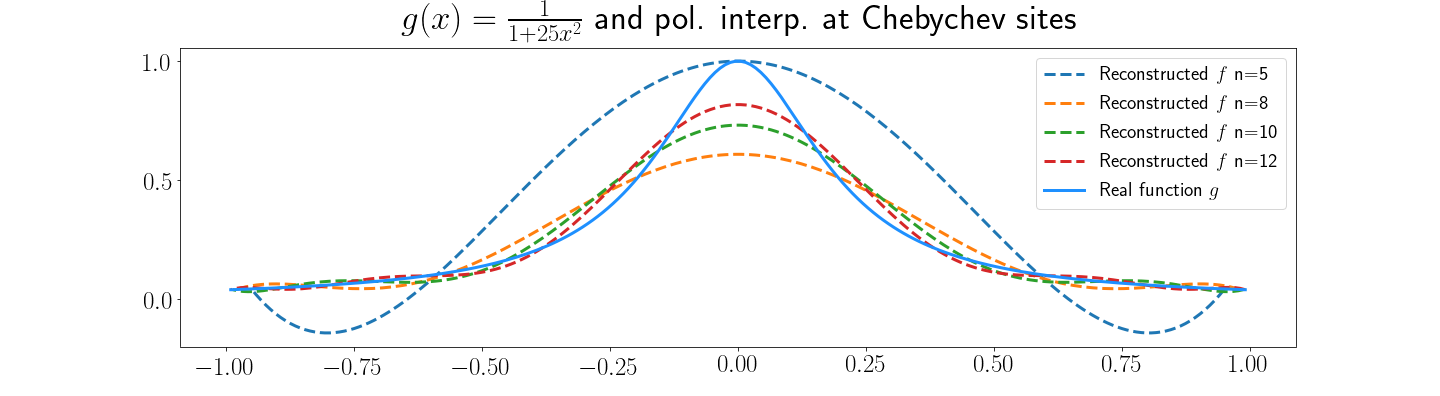
\includegraphics[width=\linewidth]{runge_2.png}
}

\frame{\frametitle{Jackson's theorem}
  \begin{thm}{2}
    If $g \in \mathcal{C}^{r}([a..b])$ and $n > r+1$ then
    \begin{equation}
      \dist(g, \Pi_{<n}) \leq const_r {\left(\frac{b-a}{n-1}\right)}^r w(g^{(r)}, \frac{b-a}{2n-1-r})
    \end{equation}
  \end{thm}

  \textbf{Idea}: break $b-a$ into $l$ pieces $x_{k+1}-x_k$ and do piecewise pol\@. approximation.\\~\\

  \underline{Pros}: multiple small polynomials instead of 1 big polynomial. \\
  \underline{Cons}: junction at breaks?
}

\subsection{I/2 Piecewise-polynomial interpolation}
\frame{\frametitle{Piecewise-linear}
  Let $t={(t_i)}_1^n$.
  \begin{itemize}
    \item $\Pi_{<k, \bm{t}}$ set of pp\@. of order k with breaks at $t_2, \ldots, t_{n-1}$. \\
    \item $S_{2,\bm{t}} = \Pi_{<2, \bm{t}} \cap \mathcal{C}^0$.  \\~\\ 
  \end{itemize}

  \pause%
  Order 2 interpolant operator $I_2:g \mapsto I_2g \in S_{2,\bm{t}}$
  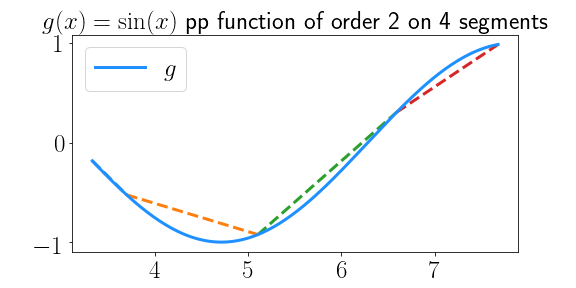
\includegraphics[width=0.5\linewidth]{pp_1.png}\hfill
  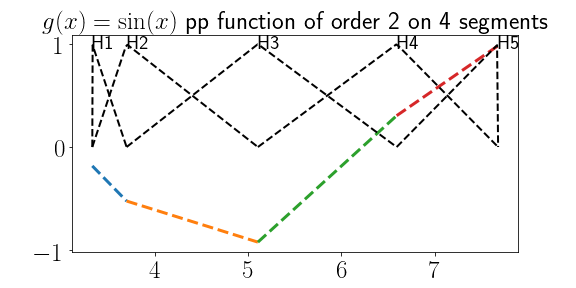
\includegraphics[width=0.5\linewidth]{pp_2.png}

  \begin{equation}
    I_2g(t) = \sum_{i=1}^n g(t_i) H_i(t)
  \end{equation}

  $(H_1, \ldots, H_n)$ is basis for $\$_{2,\bm{t}}$ 
}

%\frame{\frametitle{Piecewise cubic}
%  \begin{enumerate}
%    \item $g(t_i), \partial^1 g(t_i)$. Cubic Hermite interpolation.
%      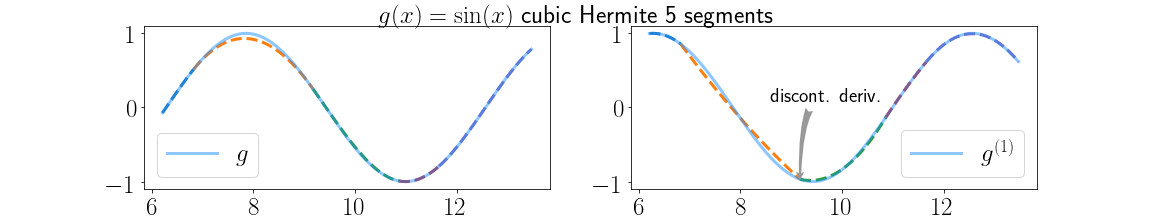
\includegraphics[width=\linewidth]{cubic_1.png}
%      \pause%
%    \item $g(t_i), \partial^1 g(t_1), \partial^1 g(t_n)$. Add  $n-2$ equations $ \partial^2 f(t_i) = \partial^2 
%      f(t_{i+1})$.  Complete Cubic spline interpolation.
%      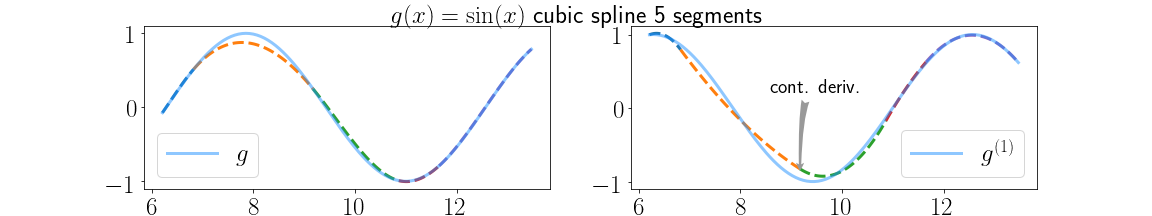
\includegraphics[width=\linewidth]{cubic_2.png}
%  \end{enumerate}
%}


%\frame{\frametitle{Piecewise cubic}
%  Let $t={(t_i)}_1^n$. The $i^{th}$ polynomial piece $\in \Pi_{<4}$ is made to satisfy
%  \begin{align}
%    f_i(t_i) &= g(t_i) & f_i(t_{i+1}) &= g(t_{i+1}) \\
%    \partial^1f_i(t_i) &= s_i & \partial^1f_i(t_{i+1}) &= s_{i+1}
%  \end{align}
%    \pause%
%    \vspace*{-5mm}
%  \begin{enumerate}
%    \item $s_i = \partial^1 g(t_i)$. Cubic Hermite interpolation.
%      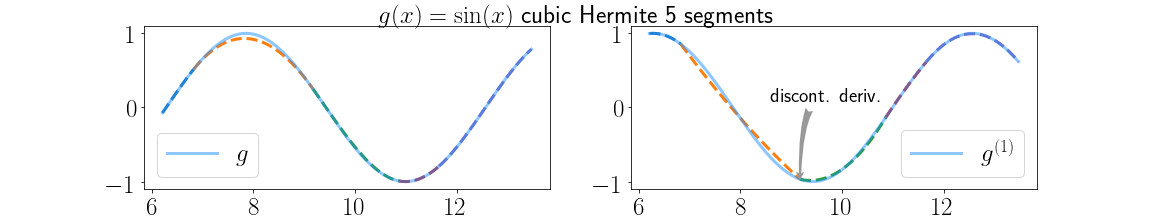
\includegraphics[width=\linewidth]{cubic_1.png}
%      \pause%
%    \item $n-2$ equations $ \partial^2 f(t_i) = \partial^2 f(t_{i+1})$. Cubic spline interpolation.
%      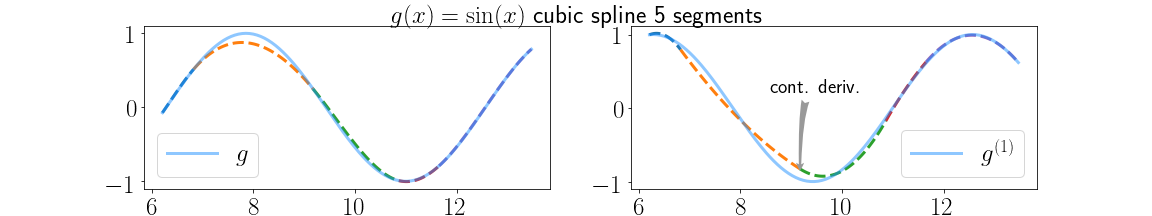
\includegraphics[width=\linewidth]{cubic_2.png}
%  \end{enumerate}
%}

\frame{\tableofcontents}

\section{II/ Introduction to spline curves}
\subsection{II/1 Cardinal B-splines}
%\frame{\frametitle{What is it?}
%%    Two equivalent definitions.
%%    \begin{deftn}{1}
%%      Let $(t_i)$ a non-decreasing sequence. The $j^{th}$ normalized B-spline of order $k$ is
%%      \begin{equation}
%%        B_{j, k, \bm{t}}(x) = (t_{j+k}-t_j)[t_j, \ldots, t_{j+k}]{(.-x)}_+^{k-1}
%%      \end{equation}
%%    \end{deftn}
%    \begin{deftn}{2}
%      Let $(t_i)$ a non-decreasing sequence. The $j^{th}$ normalized B-spline of order $k$ is given by recursive 
%      relation
%      \begin{equation}
%        B_{j, k, \bm{t}} = w_{j,k} B_{j, k-1, \bm{t}} + (1-w_{j+1,k}) B_{j+1, k-1, \bm{t}}
%      \end{equation}
%      with $w_{jk}(x) = \frac{x-t_{j}}{t_{j+k}-t_j}$ and
%        $B_{j, 1, \bm{t}}(x) = \begin{dcases}
%          1 &\text{if } t_j \leq x < t_{j+1} \\
%          0 &\text{else } \\
%        \end{dcases}$
%    \end{deftn}
%}
%
%\frame{\frametitle{Kesako?}
%  \begin{enumerate}
%    \item[1] $B_{j, k, \bm{t}}$ are in $\Pi_{<k, \bm{t}}$
%    \item[2] $B_{j, k, \bm{t}} > 0$ on $(t_j, t_{j+k})$ and $0$ outside $(t_j, t_{j+k})$
%  \end{enumerate}
%  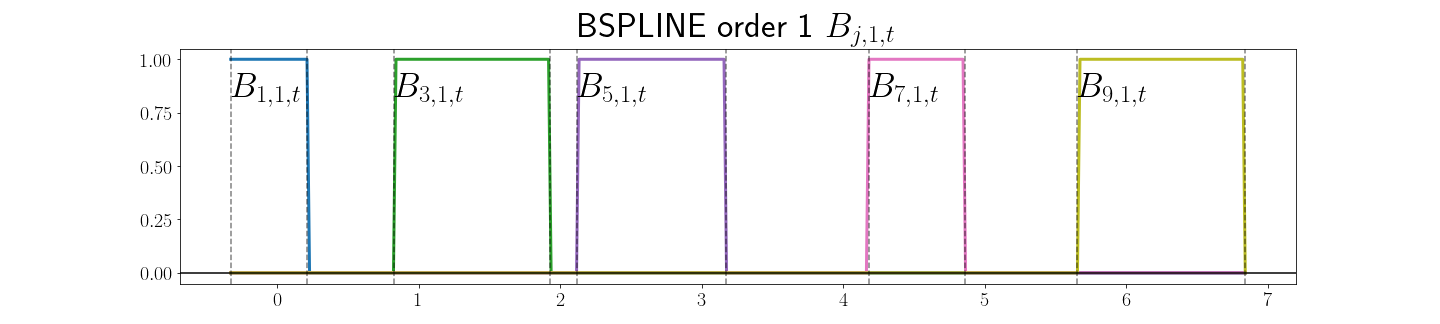
\includegraphics[width=\linewidth]{bspline_order_1.png}
%  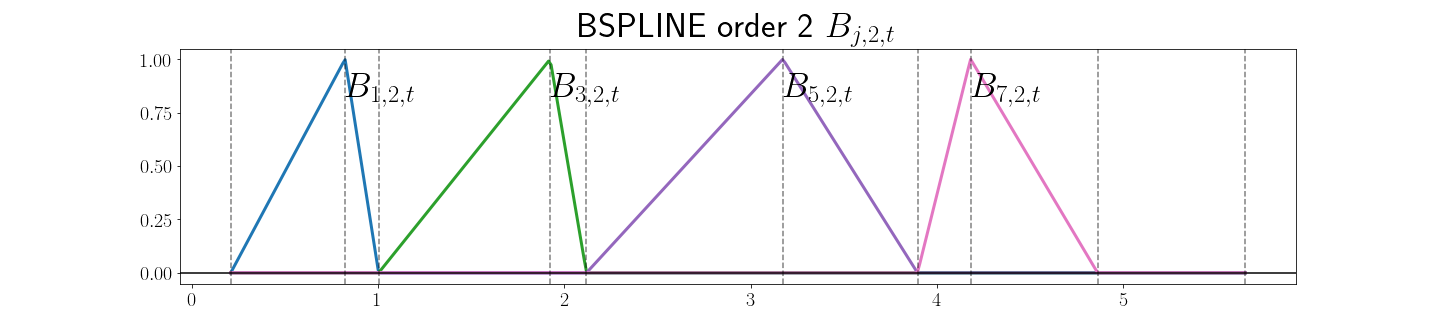
\includegraphics[width=\linewidth]{bspline_order_2.png}
%}
%
%\frame{\frametitle{Kesako?}
%  \begin{enumerate}
%    \item[3] $\sum_j B_{j, k, \bm{t}} = 1$ on $[t_k, t_{n+1}]$ (if $\bm{t} = {(t_i)}_{1}^{n+k}$)
%    \item[4] In neighborhood of $t_j$ $B_{j,k,t}$ is $\mathcal{C}^{k-1-r}$ with $r$ multiplicity of $t_j$
%  \end{enumerate}
%%  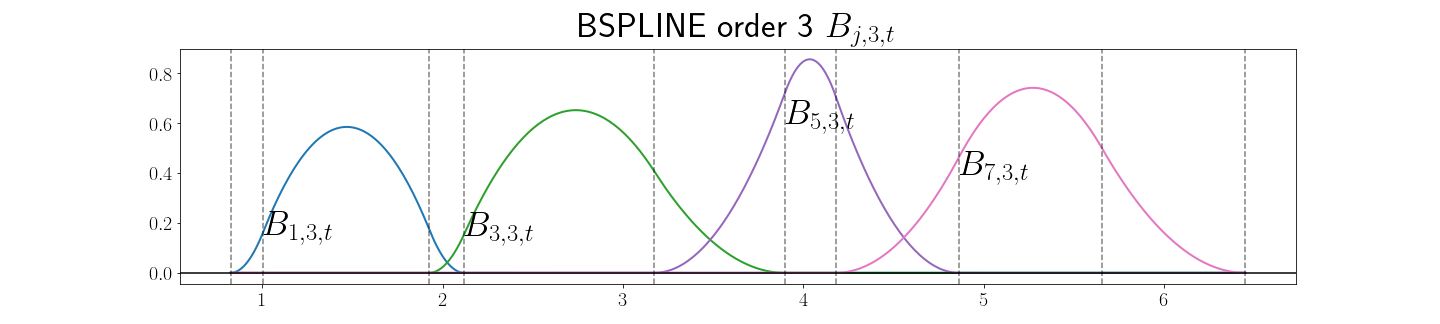
\includegraphics[width=\linewidth]{bspline_order_3.png}
%  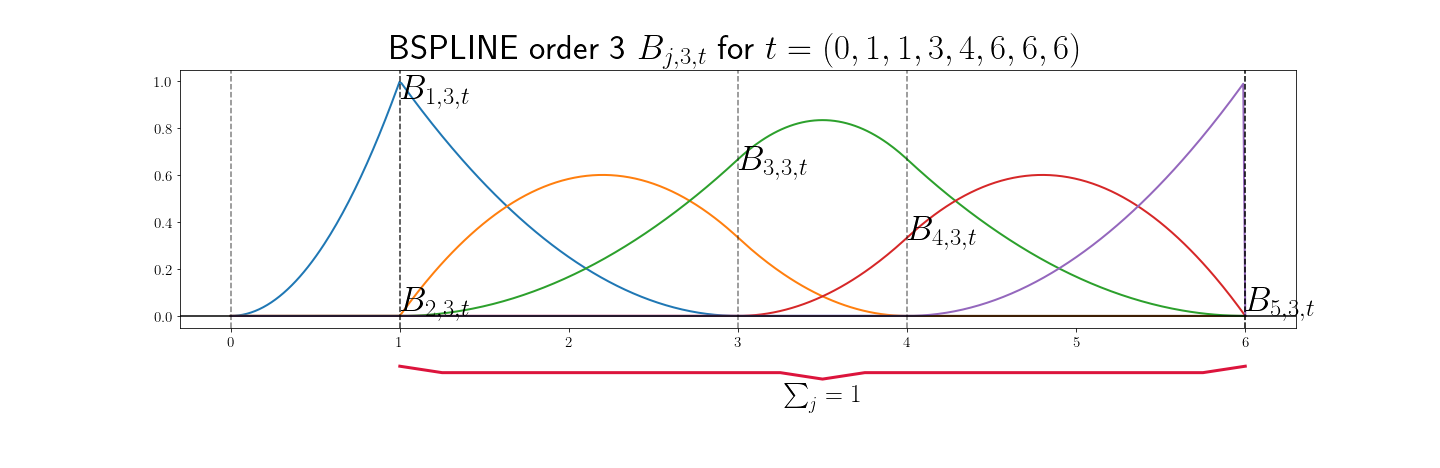
\includegraphics[width=\linewidth]{bspline_mult.png}
%  Example: knot $t_2=t_3=1$ has multiplicity 2. 
%}

\frame{\frametitle{The B-spline basis}
  \begin{deftn}{1}
    \begin{small}
    The cardinal B-spline of order $n$ (and knot multiplicity 1) is given by recursive relation
    \begin{equation}
      B^n = B^1 * B^1 * \ldots * B^1 \quad (\text{n times})
    \end{equation}
      with $B^1(t) = \begin{dcases}
          1 &\text{if } 0 \leq 1 < 1 \\
          0 &\text{else } \\
        \end{dcases}$
    \end{small}
  \end{deftn}
  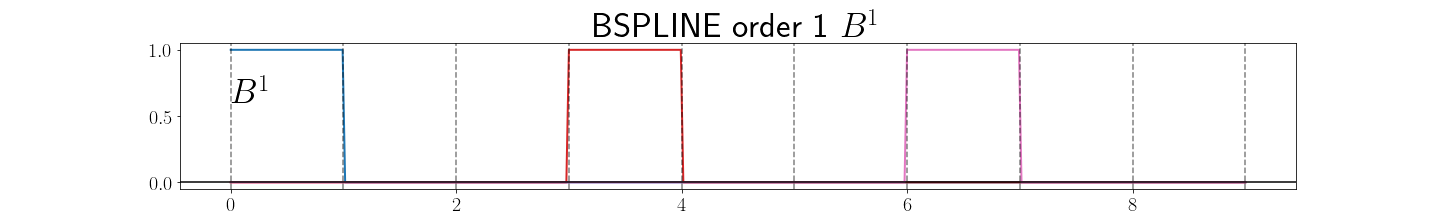
\includegraphics[width=\linewidth]{card_order_1.png}
  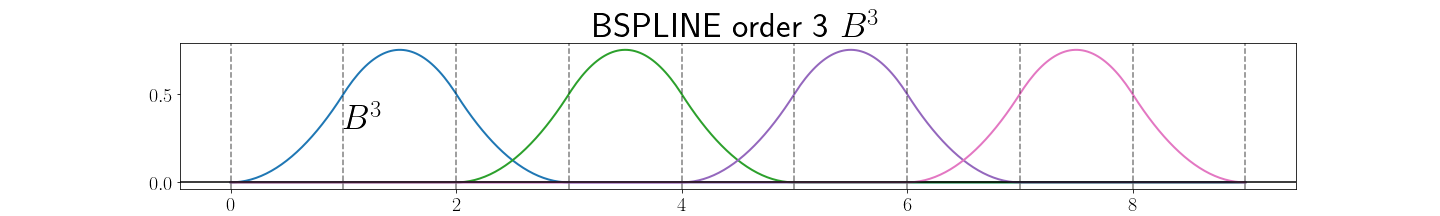
\includegraphics[width=\linewidth]{card_order_3.png}
}

\frame{\frametitle{Properties}
  Good properties
  \begin{enumerate}
    \item $B^n \in \Pi_{<n, \mathbb{Z}} \cap \mathcal{C}^{n-2}$
    \item $B^n$ is zero outside $[0,n]$
    \item (partition unity) $\displaystyle \forall t \quad \sum_{k \in \mathbb{Z}} B^n(t-k) = 1$
    \item (Riesz-basis) $\exists D_{n} \in (0,1)$ such that $\forall \bm{c}$ bounded,
      \begin{equation*}
      D_{n} \|\bm{c}\| \leq \|\sum_{k \in \mathbb{Z}} c[k] B^n(.-k) \| \leq  \|\bm{c}\|     \end{equation*}  \item 
      $\hat{B^n}(w) = {\left(\frac{1-e^{-jw}}{jw}\right)}^n$
  \end{enumerate}
}

\frame{\frametitle{Spline curve}
  \begin{deftn}{1}
    \begin{small}
    A (cardinal) \textbf{spline} or order $n$ (and knot multiplicity 1) is a linear combination of $\{B^n(.-k)\}$
    \begin{equation}
      f(t) = \sum_{k \in \mathbb{Z}} c[k] B^n(t-k)
    \end{equation}
    with $c[k] \in \mathbb{R}$. We denote $S_{n,1}$ the set of all such functions.
  \end{small}
  \end{deftn}
  \pause%
  \underline{Remarks}
  \begin{enumerate}
    \item $(c[k])$ is the sequence of \textbf{control points}.
    \item $S_{n,1} \subset \Pi_{<n, \mathbb{Z}} \cap \mathcal{C}^{n-2}$ (in fact these sets are equal!)
    \item $r_k = \#\{l| t_l = k\}$ (multiplicity), $f$ is $\mathcal{C}^{n-r_k-1}$ in $\mathcal{V}(k)$.
    \item Denote $S_{n,r}$ splines of order $n$ with knots of multiplicity $r$.
    \item A \textbf{spline curve} is a vector-valued spline i.e $c[k] \in \mathbb{R}^d$ (d=2,3 usually)
  \end{enumerate}
}

\frame{\frametitle{Dream pursued}
  Find approximation scheme $f$ interpolating $(\bm{y}_k)$
  \begin{equation}
  f(t) = \sum_{k} \bm{y}_k^T \bm{\phi}(t-t_k) \end{equation}
  and $\bm{\phi}$ retains good properties of splines (partition-unity, Riesz-basis, compact support, subdivision).
}

\subsection{II/2 Schoenberg theorems}
\frame{\frametitle{Hermite interpolation}
  Let $\mathcal{S}$ a vector space.  C.H.I.P ($y$, \ldots, $y^{(r-1)}$, $\mathcal{S}$) is solved if $\exists f \in 
  \mathcal{S}$ such that
  \begin{equation}
    \forall s=0, \ldots, r-1, \forall k \in \mathbb{Z} \qquad f^{(s)}(k) = y^{(s)}_k
  \end{equation}
    \pause%
    \begin{thm}{1}
    \begin{small}
      $n$ even, $1 \leq r \leq n/2$. The C.H.I.P ($y$, \ldots, $y^{(r-1)}$, $S_{n,r} \cap F_{\gamma, r}$ (resp.  
      $\mathcal{L}_{p,r}$)) has a unique solution iif $y^{(s)} \in Y_{\gamma}$ (resp. $l_p$). \underline{In that case}
    \begin{equation}
      f(t) = \sum_{k \in \mathbb{Z}} y_k L_{n,r,0}(t-k) + \ldots, y^{(r-1)}_k L_{n,r-1}(t-k)
    \end{equation}
  \end{small}
 \end{thm}
 \underline{Remarks}
 \begin{enumerate}
   \item $L_{n,r,s}$ are elements of $S_{n,r}$. Calculated by solving system of $n-r$ equations.
   \item $f \in S_{n,r}$ is a \textbf{spline} of order $n$
 \end{enumerate}
}

\frame{\frametitle{Hermite snakes (Uhlmann 2016)}
  \underline{Data}: at $M$ sites ${\{r[k]\}}_{k=0}^{M-1},{\{r'[k]\}}_{k=0}^{M-1}$. \\
  \underline{Obj}: Continuous representation of the curve $r(t) = (r_1(t), r_2(t))$ \\
  \pause%
  \smallbreak%
  Schoenberg for $n=4$ and $r=2$\\
  \begin{equation}
    r(t) = \sum_{k \in \mathbb{Z}} r[k] \phi_1(t-k) + r'[k] \phi_2(t-k)
  \end{equation}
    
  $\phi_1 = L_{4, 2, 0}, \phi_2 = L_{4,2,1}$ (polynomials order 4). $r_1, r_2 \in \mathcal{C}^{n-r-1} = \mathcal{C}^1$.
  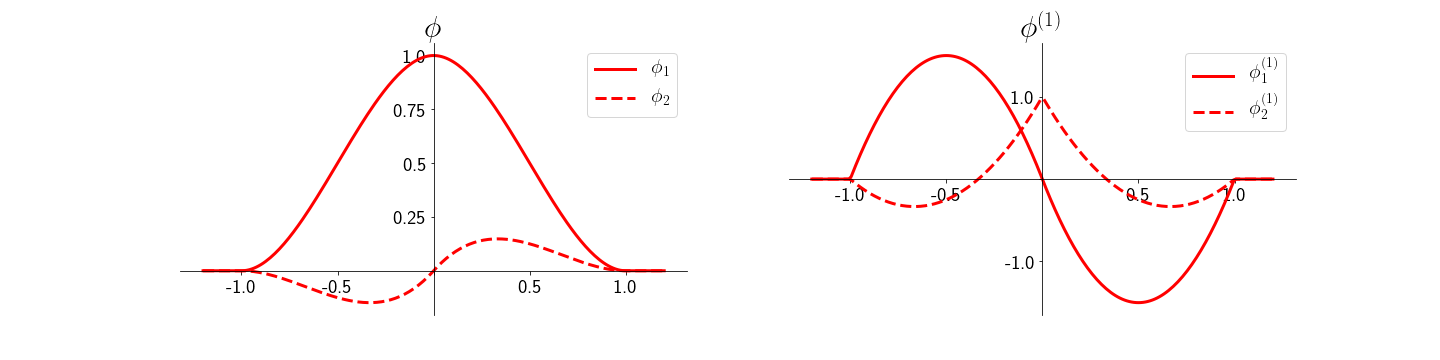
\includegraphics[width=\linewidth]{hermite_uhl.png}
}

\frame{\frametitle{Hermite snakes (Uhlmann 2016)}
  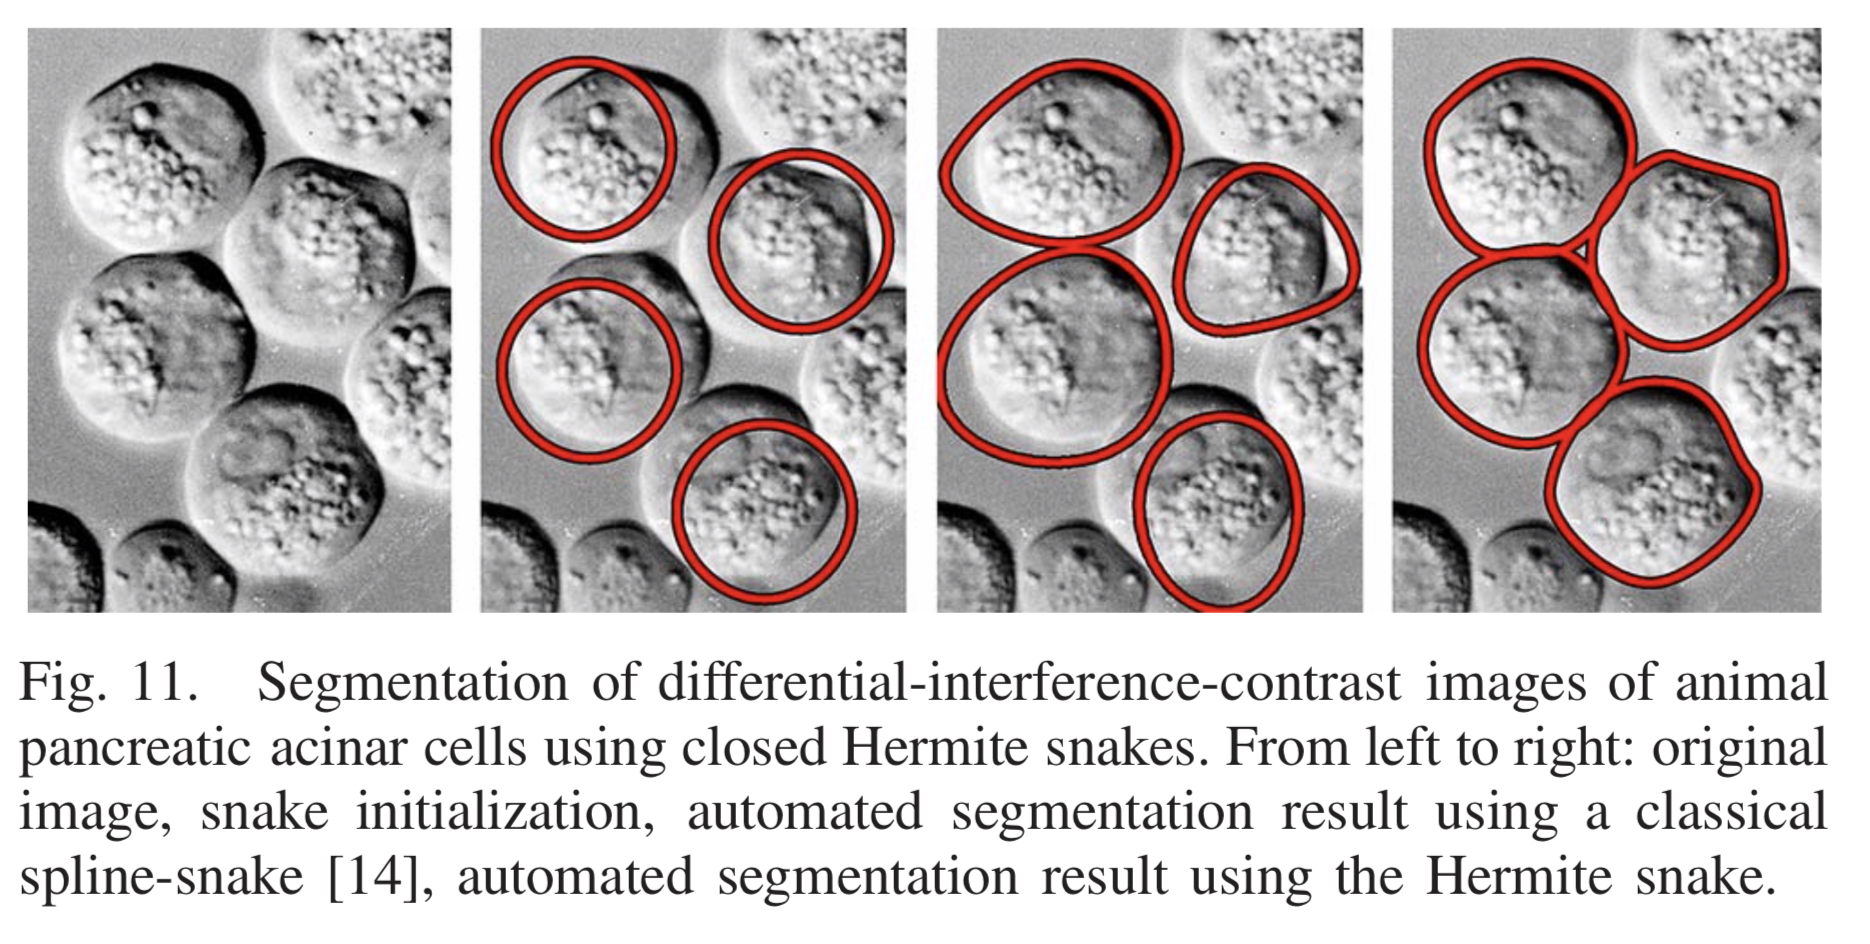
\includegraphics[width=\linewidth]{hermite_ex.png}
}

\subsection{II/3 Ellipse-preserving snakes}
\frame{\frametitle{Ellipse-preserving Hermite (Conti 2015)}
  \underline{Data}: at $M$ sites ${\{r[k]\}}_{k=0}^{M-1},{\{r'[k]\}}_{k=0}^{M-1}$. \\
  \underline{Obj}: Continuous representation of the curve $r(t) = (r_1(t), r_2(t))$. Good basis and \textbf{reproduction 
  of unit circle.}
  \pause%
  \begin{equation}
    \quad r(t) = \sum_{k \in \mathbb{Z}} r[k] \phi_1(t-k) + r'[k] \phi_2(t-k)
  \end{equation}
  
  with $\phi_i(t) = \left(a_i(t) + b_i(t)t + c_i(t) e^{jwx} + d_i(t) e^{-jwx}\right) \chi_{[-1,1]}$ and $w = 
  \frac{2\pi}{M}$ (exponential polynomials).\\
  \medbreak%
  \underline{Remark}: here the curve is said to be an \textbf{exponential spline curve}
}

\frame{\frametitle{Ellipse-preserving Hermite (Conti 2015)}
  Reproducing sinusoids with $M$ coefficients
  \begin{align}
    \cos (2\pi t) &= \sum_{k \in \mathbb{Z}} \cos (\frac{2\pi k}{M}) \phi_1(Mt-k) - \frac{2\pi}{M} \sin (\frac{2\pi 
    k}{M}) \phi_2(Mt-k) \\
  \sin (2\pi t) &= \sum_{k \in \mathbb{Z}} \sin (\frac{2\pi k}{M}) \phi_1(Mt-k) + \frac{2\pi k}{M} \cos (\frac{2\pi 
  k}{M}) \phi_2(Mt-k)
  \end{align}
  }

\frame{\tableofcontents}

\section{III/ Representation of spline surfaces}
\subsection{III/1 Extension of Conti's scheme}
\frame{\frametitle{The case of the unit sphere}
  The sphere surface parametrized by $g=\sigma: \mathbb{R}^2 \to \mathbb{R}^3$
  \begin{equation}
    \sigma(u,v) = \begin{bmatrix} \cos(2\pi u)\sin(\pi v) \\ \sin(2\pi u)\sin(\pi v) \\ \cos(\pi v) \end{bmatrix} \quad 
    (u, v) \in {[0,1]}^2
  \end{equation}
  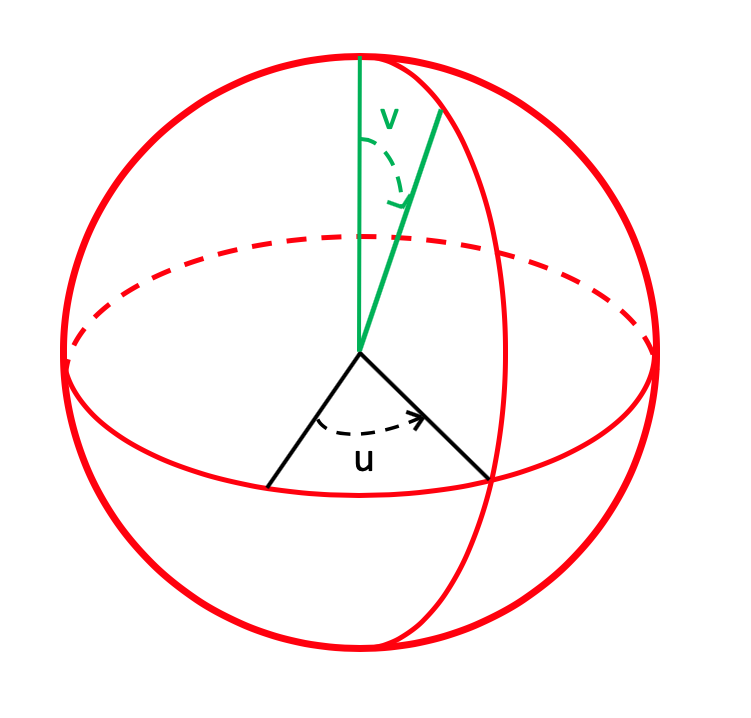
\includegraphics[width=0.4\linewidth]{sphere_param.png}
}

\frame{\frametitle{From 2D to 3D for tensor-product surfaces}
  \underline{Data}: $M_1$ control points on latitudes, $M_2+1$ control points on longitudes. At each point $4$ 
  parameters $\sigma, \partial^{1,0} \sigma, \partial^{0,1} \sigma, \partial^{1,1} \sigma$. \\
  \underline{Obj}: Continuous representation of $g:\mathbb{R}^2 \to \mathbb{R}^3$ \\
  \pause%
    \begin{align*}
      \sigma(u,v) &= \sum_{k=0}^{M_1-1} \sum_{l=0}^{M_2} c_1[k,l]\phi_{1, w_1, per}(M_1u-k)\phi_{1, w_2}(M_2v-l) \\
      &+ \sum_{k=0}^{M_1-1} \sum_{l=0}^{M_2} c_2[k,l] \phi_{1, w_1, per}(M_1u-k)\phi_{2, w_2}(M_2v-l) \\
      &+ \sum_{k=0}^{M_1-1} \sum_{l=0}^{M_2} c_3[k,l] \phi_{2, w_1, per}(M_1u-k)\phi_{1, w_2}(M_2v-l) \\
      &+ \sum_{k=0}^{M_1-1} \sum_{l=0}^{M_2} c_4[k,l] \phi_{2, w_1, per}(M_1u-k)\phi_{2, w_2}(M_2v-l) \\
    \end{align*}
  }

\frame{\frametitle{From 2D to 3D for tensor-product surfaces}  \begin{align*}
  c_1[k,l] &= \sigma(\frac{k}{M_1},\frac{l}{M_2}) & c_2[k,l] &= \frac{1}{M_2}\frac{\partial \sigma}{\partial 
  v}(\frac{k}{M_1}, \frac{l}{M_2}) \\
  c_3[k,l] &= \frac{1}{M_1} \frac{\partial \sigma}{\partial u}(\frac{k}{M_1}, \frac{l}{M_2}) &
  c_4[k,l] &= \frac{1}{M_1 M_2} \frac{\partial^2 \sigma}{\partial u \partial v}(\frac{k}{M_1}, \frac{l}{M_2})
   \end{align*}

   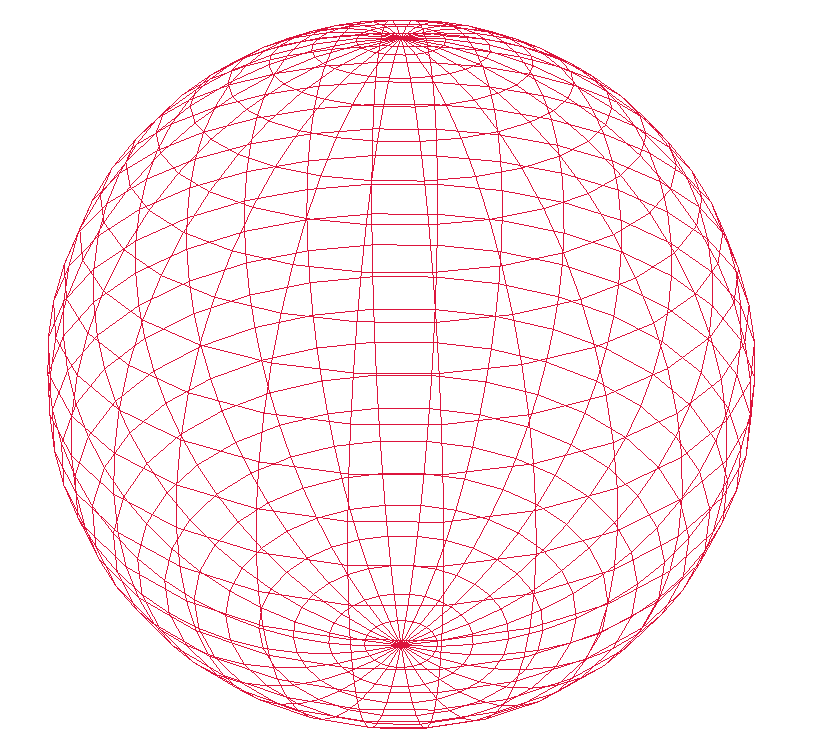
\includegraphics[width=0.4\linewidth]{sphere_vtk.png}\hfill
   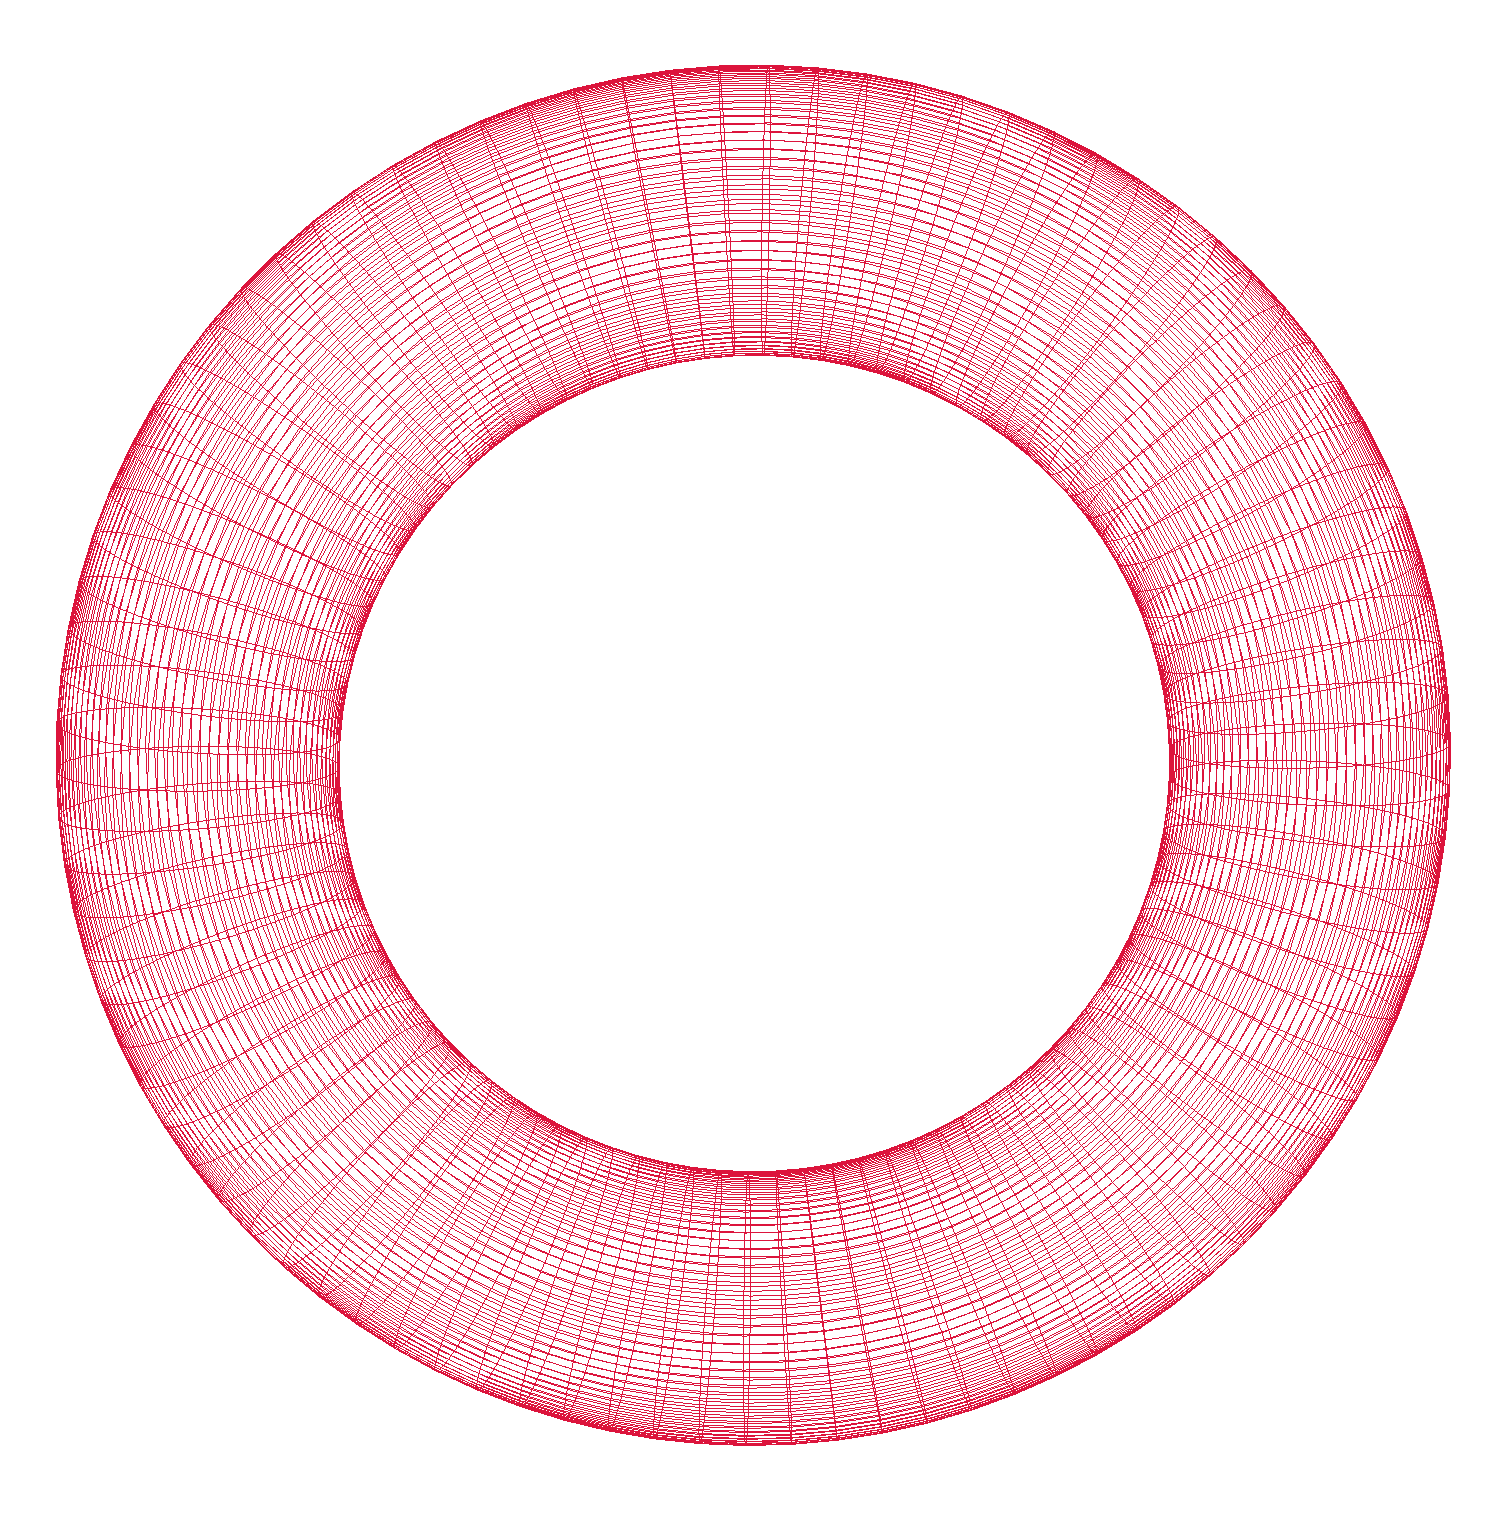
\includegraphics[width=0.4\linewidth]{torus_vtk.png}
}

\subsection{III/2 The twist vector}
\frame{\frametitle{Mysterious twist vector}
   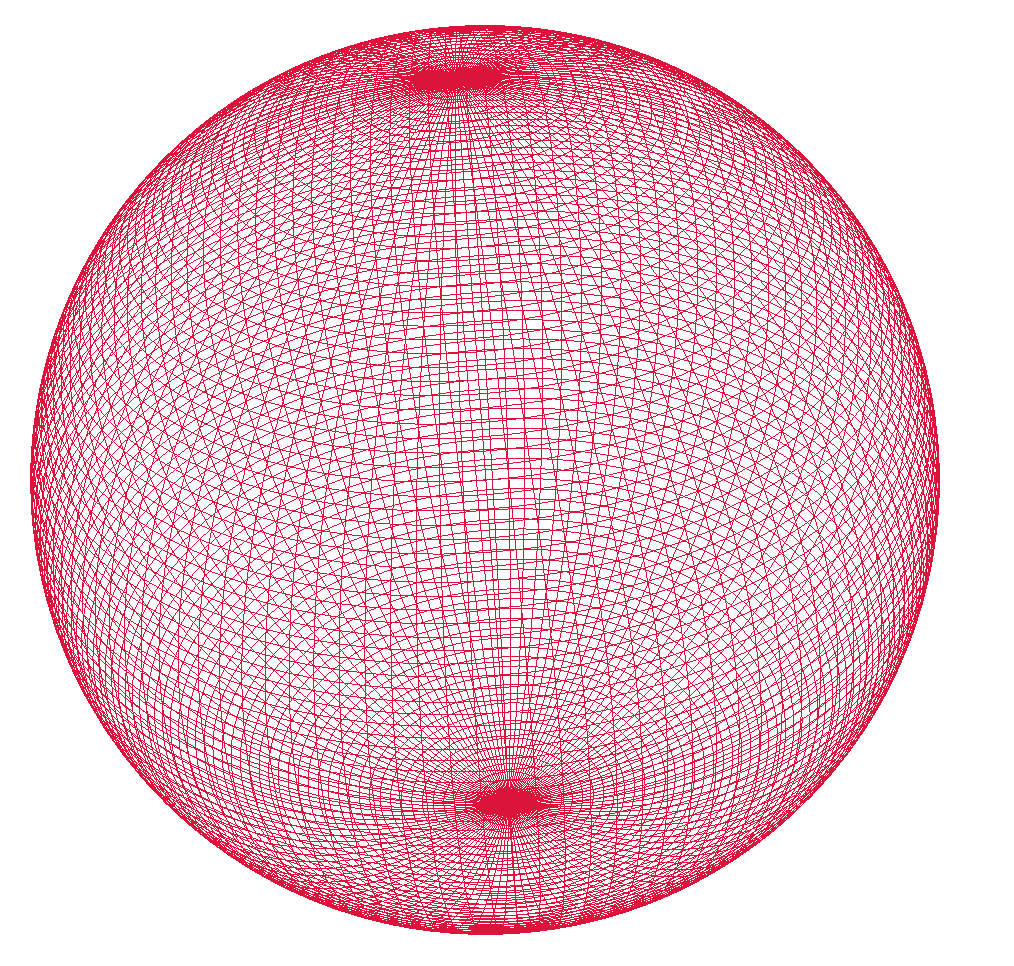
\includegraphics[width=0.5\linewidth]{sphere_twist.png}\hfill
   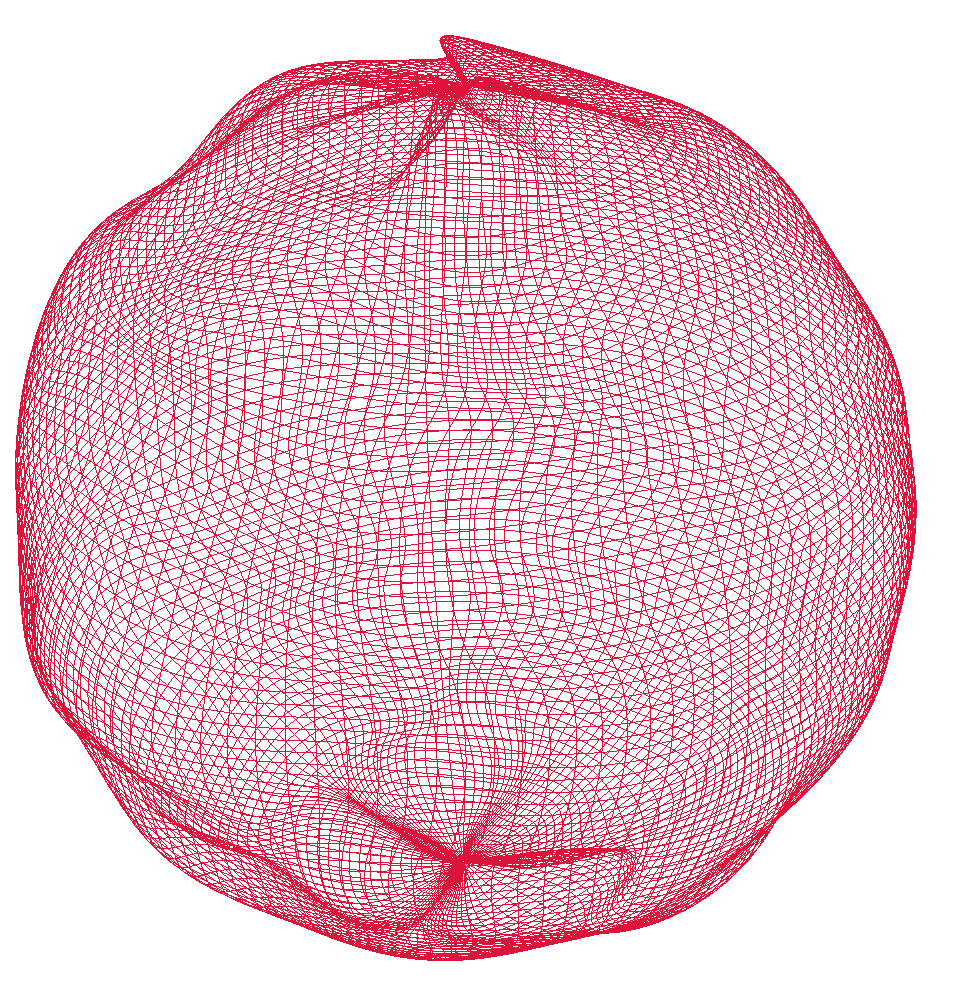
\includegraphics[width=0.5\linewidth]{sphere_twist_rand.png}
}

\section{Summary and future research}
\frame{\frametitle{Summary and what next}
  \underline{Take-away}
  \begin{enumerate}
       \item How to go from discrete to continuous
       \item What are spline curves
       \item What is a good basis
  \end{enumerate}
  \pause%
  \underline{Ongoing}
  \begin{enumerate}
    \item Estimation of not intuitive parameters
    \item Second-order Hermite interpolation
    \item What basis for what purpose
  \end{enumerate}
}

\end{document}
